% Created by tikzDevice version 0.6.2-92-0ad2792 on 2012-11-09 11:12:14
% !TEX encoding = UTF-8 Unicode
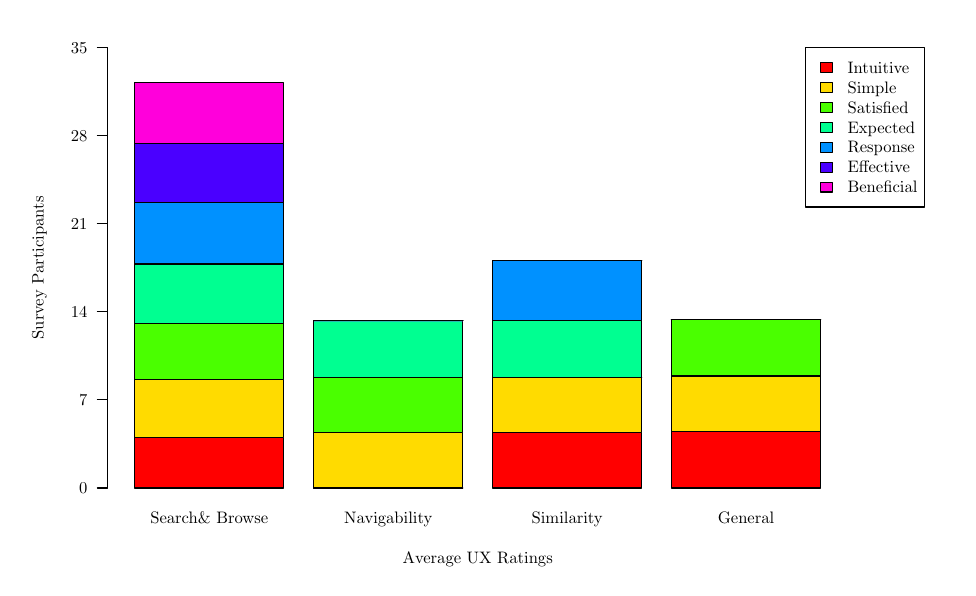
\begin{tikzpicture}[x=1pt,y=1pt]
\definecolor[named]{fillColor}{rgb}{1.00,1.00,1.00}
\path[use as bounding box,fill=fillColor,fill opacity=0.00] (0,0) rectangle (332.44,195.13);
\begin{scope}
\path[clip] (  0.00,  0.00) rectangle (332.44,195.13);
\definecolor[named]{drawColor}{rgb}{0.00,0.00,0.00}
\definecolor[named]{fillColor}{rgb}{1.00,0.00,0.00}

\path[draw=drawColor,line width= 0.4pt,line join=round,line cap=round,fill=fillColor] ( 38.71, 28.80) rectangle ( 92.59, 46.99);
\definecolor[named]{fillColor}{rgb}{1.00,0.86,0.00}

\path[draw=drawColor,line width= 0.4pt,line join=round,line cap=round,fill=fillColor] ( 38.71, 46.99) rectangle ( 92.59, 67.90);
\definecolor[named]{fillColor}{rgb}{0.29,1.00,0.00}

\path[draw=drawColor,line width= 0.4pt,line join=round,line cap=round,fill=fillColor] ( 38.71, 67.90) rectangle ( 92.59, 88.36);
\definecolor[named]{fillColor}{rgb}{0.00,1.00,0.57}

\path[draw=drawColor,line width= 0.4pt,line join=round,line cap=round,fill=fillColor] ( 38.71, 88.36) rectangle ( 92.59,109.73);
\definecolor[named]{fillColor}{rgb}{0.00,0.57,1.00}

\path[draw=drawColor,line width= 0.4pt,line join=round,line cap=round,fill=fillColor] ( 38.71,109.73) rectangle ( 92.59,132.01);
\definecolor[named]{fillColor}{rgb}{0.29,0.00,1.00}

\path[draw=drawColor,line width= 0.4pt,line join=round,line cap=round,fill=fillColor] ( 38.71,132.01) rectangle ( 92.59,153.38);
\definecolor[named]{fillColor}{rgb}{1.00,0.00,0.86}

\path[draw=drawColor,line width= 0.4pt,line join=round,line cap=round,fill=fillColor] ( 38.71,153.38) rectangle ( 92.59,175.20);
\definecolor[named]{fillColor}{rgb}{1.00,0.00,0.00}

\path[draw=drawColor,line width= 0.4pt,line join=round,line cap=round,fill=fillColor] (103.36, 28.80) rectangle (157.23, 28.80);
\definecolor[named]{fillColor}{rgb}{1.00,0.86,0.00}

\path[draw=drawColor,line width= 0.4pt,line join=round,line cap=round,fill=fillColor] (103.36, 28.80) rectangle (157.23, 48.80);
\definecolor[named]{fillColor}{rgb}{0.29,1.00,0.00}

\path[draw=drawColor,line width= 0.4pt,line join=round,line cap=round,fill=fillColor] (103.36, 48.80) rectangle (157.23, 68.81);
\definecolor[named]{fillColor}{rgb}{0.00,1.00,0.57}

\path[draw=drawColor,line width= 0.4pt,line join=round,line cap=round,fill=fillColor] (103.36, 68.81) rectangle (157.23, 89.27);
\definecolor[named]{fillColor}{rgb}{0.00,0.57,1.00}

\path[draw=drawColor,line width= 0.4pt,line join=round,line cap=round,fill=fillColor] (103.36, 89.27) rectangle (157.23, 89.27);
\definecolor[named]{fillColor}{rgb}{0.29,0.00,1.00}

\path[draw=drawColor,line width= 0.4pt,line join=round,line cap=round,fill=fillColor] (103.36, 89.27) rectangle (157.23, 89.27);
\definecolor[named]{fillColor}{rgb}{1.00,0.00,0.86}

\path[draw=drawColor,line width= 0.4pt,line join=round,line cap=round,fill=fillColor] (103.36, 89.27) rectangle (157.23, 89.27);
\definecolor[named]{fillColor}{rgb}{1.00,0.00,0.00}

\path[draw=drawColor,line width= 0.4pt,line join=round,line cap=round,fill=fillColor] (168.01, 28.80) rectangle (221.88, 48.80);
\definecolor[named]{fillColor}{rgb}{1.00,0.86,0.00}

\path[draw=drawColor,line width= 0.4pt,line join=round,line cap=round,fill=fillColor] (168.01, 48.80) rectangle (221.88, 68.81);
\definecolor[named]{fillColor}{rgb}{0.29,1.00,0.00}

\path[draw=drawColor,line width= 0.4pt,line join=round,line cap=round,fill=fillColor] (168.01, 68.81) rectangle (221.88, 68.81);
\definecolor[named]{fillColor}{rgb}{0.00,1.00,0.57}

\path[draw=drawColor,line width= 0.4pt,line join=round,line cap=round,fill=fillColor] (168.01, 68.81) rectangle (221.88, 89.27);
\definecolor[named]{fillColor}{rgb}{0.00,0.57,1.00}

\path[draw=drawColor,line width= 0.4pt,line join=round,line cap=round,fill=fillColor] (168.01, 89.27) rectangle (221.88,111.09);
\definecolor[named]{fillColor}{rgb}{0.29,0.00,1.00}

\path[draw=drawColor,line width= 0.4pt,line join=round,line cap=round,fill=fillColor] (168.01,111.09) rectangle (221.88,111.09);
\definecolor[named]{fillColor}{rgb}{1.00,0.00,0.86}

\path[draw=drawColor,line width= 0.4pt,line join=round,line cap=round,fill=fillColor] (168.01,111.09) rectangle (221.88,111.09);
\definecolor[named]{fillColor}{rgb}{1.00,0.00,0.00}

\path[draw=drawColor,line width= 0.4pt,line join=round,line cap=round,fill=fillColor] (232.66, 28.80) rectangle (286.53, 49.26);
\definecolor[named]{fillColor}{rgb}{1.00,0.86,0.00}

\path[draw=drawColor,line width= 0.4pt,line join=round,line cap=round,fill=fillColor] (232.66, 49.26) rectangle (286.53, 69.26);
\definecolor[named]{fillColor}{rgb}{0.29,1.00,0.00}

\path[draw=drawColor,line width= 0.4pt,line join=round,line cap=round,fill=fillColor] (232.66, 69.26) rectangle (286.53, 89.72);
\definecolor[named]{fillColor}{rgb}{0.00,1.00,0.57}

\path[draw=drawColor,line width= 0.4pt,line join=round,line cap=round,fill=fillColor] (232.66, 89.72) rectangle (286.53, 89.72);
\definecolor[named]{fillColor}{rgb}{0.00,0.57,1.00}

\path[draw=drawColor,line width= 0.4pt,line join=round,line cap=round,fill=fillColor] (232.66, 89.72) rectangle (286.53, 89.72);
\definecolor[named]{fillColor}{rgb}{0.29,0.00,1.00}

\path[draw=drawColor,line width= 0.4pt,line join=round,line cap=round,fill=fillColor] (232.66, 89.72) rectangle (286.53, 89.72);
\definecolor[named]{fillColor}{rgb}{1.00,0.00,0.86}

\path[draw=drawColor,line width= 0.4pt,line join=round,line cap=round,fill=fillColor] (232.66, 89.72) rectangle (286.53, 89.72);
\end{scope}
\begin{scope}
\path[clip] (  0.00,  0.00) rectangle (332.44,195.13);
\definecolor[named]{drawColor}{rgb}{0.00,0.00,0.00}

\node[text=drawColor,anchor=base,inner sep=0pt, outer sep=0pt, scale=  0.60] at ( 65.65, 15.84) {Search\& Browse};

\node[text=drawColor,anchor=base,inner sep=0pt, outer sep=0pt, scale=  0.60] at (130.30, 15.84) {Navigability};

\node[text=drawColor,anchor=base,inner sep=0pt, outer sep=0pt, scale=  0.60] at (194.94, 15.84) {Similarity};

\node[text=drawColor,anchor=base,inner sep=0pt, outer sep=0pt, scale=  0.60] at (259.59, 15.84) {General};
\end{scope}
\begin{scope}
\path[clip] (  0.00,  0.00) rectangle (332.44,195.13);
\definecolor[named]{drawColor}{rgb}{0.00,0.00,0.00}

\node[text=drawColor,anchor=base,inner sep=0pt, outer sep=0pt, scale=  0.60] at (162.62,  1.44) {Average UX Ratings};

\node[text=drawColor,rotate= 90.00,anchor=base,inner sep=0pt, outer sep=0pt, scale=  0.60] at (  5.76,108.36) {Survey Participants};
\end{scope}
\begin{scope}
\path[clip] (  0.00,  0.00) rectangle (332.44,195.13);
\definecolor[named]{drawColor}{rgb}{0.00,0.00,0.00}

\path[draw=drawColor,line width= 0.4pt,line join=round,line cap=round] ( 28.80, 28.80) -- ( 28.80,187.93);

\path[draw=drawColor,line width= 0.4pt,line join=round,line cap=round] ( 28.80, 28.80) -- ( 25.20, 28.80);

\path[draw=drawColor,line width= 0.4pt,line join=round,line cap=round] ( 28.80, 60.63) -- ( 25.20, 60.63);

\path[draw=drawColor,line width= 0.4pt,line join=round,line cap=round] ( 28.80, 92.45) -- ( 25.20, 92.45);

\path[draw=drawColor,line width= 0.4pt,line join=round,line cap=round] ( 28.80,124.28) -- ( 25.20,124.28);

\path[draw=drawColor,line width= 0.4pt,line join=round,line cap=round] ( 28.80,156.10) -- ( 25.20,156.10);

\path[draw=drawColor,line width= 0.4pt,line join=round,line cap=round] ( 28.80,187.93) -- ( 25.20,187.93);

\node[text=drawColor,anchor=base east,inner sep=0pt, outer sep=0pt, scale=  0.60] at ( 21.60, 26.73) {0};

\node[text=drawColor,anchor=base east,inner sep=0pt, outer sep=0pt, scale=  0.60] at ( 21.60, 58.56) {7};

\node[text=drawColor,anchor=base east,inner sep=0pt, outer sep=0pt, scale=  0.60] at ( 21.60, 90.39) {14};

\node[text=drawColor,anchor=base east,inner sep=0pt, outer sep=0pt, scale=  0.60] at ( 21.60,122.21) {21};

\node[text=drawColor,anchor=base east,inner sep=0pt, outer sep=0pt, scale=  0.60] at ( 21.60,154.04) {28};

\node[text=drawColor,anchor=base east,inner sep=0pt, outer sep=0pt, scale=  0.60] at ( 21.60,185.86) {35};
\end{scope}
\begin{scope}
\path[clip] (  0.00,  0.00) rectangle (332.44,195.13);
\definecolor[named]{drawColor}{rgb}{0.00,0.00,0.00}

\path[draw=drawColor,line width= 0.4pt,line join=round,line cap=round] (281.14,187.93) rectangle (324.21,130.33);
\definecolor[named]{fillColor}{rgb}{1.00,0.00,0.00}

\path[draw=drawColor,line width= 0.4pt,line join=round,line cap=round,fill=fillColor] (286.54,182.53) rectangle (290.86,178.93);
\definecolor[named]{fillColor}{rgb}{1.00,0.86,0.00}

\path[draw=drawColor,line width= 0.4pt,line join=round,line cap=round,fill=fillColor] (286.54,175.33) rectangle (290.86,171.73);
\definecolor[named]{fillColor}{rgb}{0.29,1.00,0.00}

\path[draw=drawColor,line width= 0.4pt,line join=round,line cap=round,fill=fillColor] (286.54,168.13) rectangle (290.86,164.53);
\definecolor[named]{fillColor}{rgb}{0.00,1.00,0.57}

\path[draw=drawColor,line width= 0.4pt,line join=round,line cap=round,fill=fillColor] (286.54,160.93) rectangle (290.86,157.33);
\definecolor[named]{fillColor}{rgb}{0.00,0.57,1.00}

\path[draw=drawColor,line width= 0.4pt,line join=round,line cap=round,fill=fillColor] (286.54,153.73) rectangle (290.86,150.13);
\definecolor[named]{fillColor}{rgb}{0.29,0.00,1.00}

\path[draw=drawColor,line width= 0.4pt,line join=round,line cap=round,fill=fillColor] (286.54,146.53) rectangle (290.86,142.93);
\definecolor[named]{fillColor}{rgb}{1.00,0.00,0.86}

\path[draw=drawColor,line width= 0.4pt,line join=round,line cap=round,fill=fillColor] (286.54,139.33) rectangle (290.86,135.73);

\node[text=drawColor,anchor=base west,inner sep=0pt, outer sep=0pt, scale=  0.60] at (296.26,178.66) {Intuitive};

\node[text=drawColor,anchor=base west,inner sep=0pt, outer sep=0pt, scale=  0.60] at (296.26,171.46) {Simple};

\node[text=drawColor,anchor=base west,inner sep=0pt, outer sep=0pt, scale=  0.60] at (296.26,164.26) {Satisfied};

\node[text=drawColor,anchor=base west,inner sep=0pt, outer sep=0pt, scale=  0.60] at (296.26,157.06) {Expected};

\node[text=drawColor,anchor=base west,inner sep=0pt, outer sep=0pt, scale=  0.60] at (296.26,149.86) {Response};

\node[text=drawColor,anchor=base west,inner sep=0pt, outer sep=0pt, scale=  0.60] at (296.26,142.66) {Effective};

\node[text=drawColor,anchor=base west,inner sep=0pt, outer sep=0pt, scale=  0.60] at (296.26,135.46) {Beneficial};
\end{scope}
\end{tikzpicture}
